
% chapter one: dark matter?
%\begin{document}

\chapter{The Case for Dark Matter}

For most of the last century evidence for the existence of dark matter has been gathering from various sources. Initially, evidence was primarily from astrophysical observations of the behaviour of various structures observed in the universe. However, once cosmology became a predictive tool, more stringent requirements could be placed on the unseen parts of the universe. We will begin by evaluating the astrophysical and cosmological evidences for the existence of dark matter, and discussing some proposed models.

\section{Astrophysical Evidence for Dark Matter}

The first indications that something was amiss in astronomy was from observations made of what was then the Andromeda Nebula by Heber Curtis in 1917~\cite{}. Based on these observations, Curtis concluded that the Nebula was actually an entirely separate galaxy at some immense distance from the Milky Way. In the 1920s Edwin Hubble showed conclusively that the universe was much more than just our Milky Way galaxy~\cite{Hubble:1929}. The next logical step was for astronomers to study this recently-discovered rest of the universe. Very soon it became clear that there was a great deal about which we knew very little.

\subsection{Rotation curves}

In the early 17th century Johannes Kepler published his three laws of planetary motion \cite{Kepler}. Kepler's Third law gives a relationship between an orbit's period, semimajor axis (radius, if circular), and enclosed mass. Assuming the mass distribution is a function purely of radius, we can define
\begin{equation} \label{eq:mass_distribution}
M(r) = \int_0^r \n{d}^3r'\, \rho (r') = 4\pi\,\int_0^r \n{d}r'\, r'^{2} \rho(r')
\end{equation}
We can do a bit of manipulation on the expression Kepler found to give us a relationship relating the expected orbital velocity of an object in a galaxy as a function of its distance from the galactic core,
\begin{equation} \label{eq:rotation_curve}
v(r) = \sqrt{\frac{GM(r)}{r}}
\end{equation}

Armed with~\eqref{eq:mass_distribtion} and~\eqref{eq:rotation_curve}, we can calculate $M(r)$ by observing a galaxy with telescopes and assuming some stellar mass distribution, and then make some prediction for $v(r)$. Using Doppler-shifted lines of stars or dwarf galaxies, the orbital velocities can be measured and compared to the prediction from the mass distribution. The predicted and measured rotation speeds bear only marginal resemblances to each other, as seen in figure~\ref{fig:rotation_curve}, an image of the Triangulum galaxy (M33).

\begin{figure}[h]
	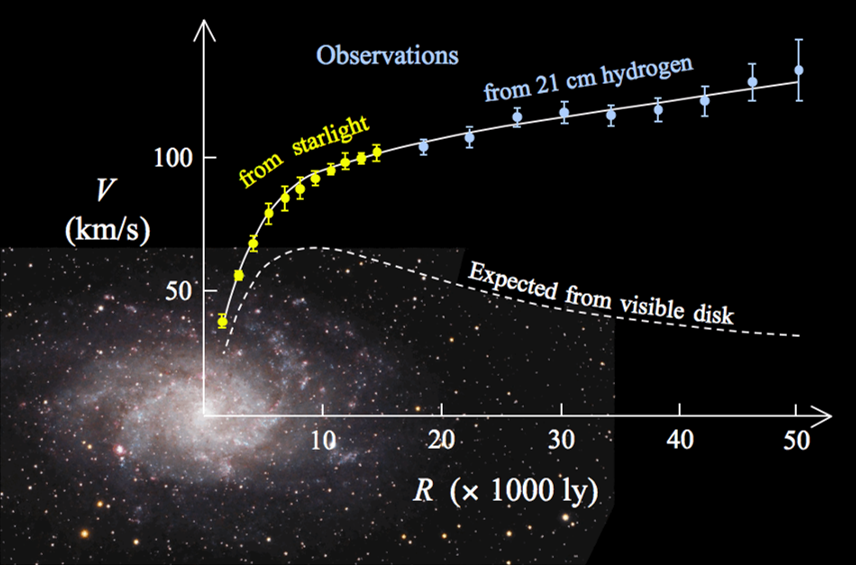
\includegraphics{figures/chapter_one/rotation_curve.png}
	\caption{Rotation curve of M33, from~\cite{Corbelli:1999af}}
	\label{fig:rotation_curve}
\end{figure}

Clearly, something is wrong with the predictions. If we assume that stars, gas, dust, and other objects visible with telescopes are all there is to a galaxy, then at large distances from the galactic center it will increasingly appear like a point mass, giving the familiar relationship $v(r) ~ r^{-1/2}$ that is Kepler's third law. In the bulge in the center of the galaxy, we see the speed increases roughly linearly with the radius, indicating a mass distribution proportional to $r^3$, or a constant density profile. However, the data clearly shows that at large $r$, the velocity is approximately constant, indicating a mass distribution proportional to $r$ or a density profile proportional to $1/r^2$. If there is something in the galaxy that would produce this distribution of mass it doesn't show up in any telescope. Additionally, the stars near the edge of the galaxy are well above the predicted escape velocity $v_{\n{esc}} = \sqrt{2}v_{\n{circ}}$, and as galaxies are stable over astronomical periods of time, they cannot be filled with objects exceding the escape velocity.

This data indicate one of two things. Either Kepler's Law and the Newtonian gravity upon which it is based are invalid on galactic distance scales, or there is some hidden mass or dark matter filling a galaxy. Supposing the first case to be true, the recourse would be to introduce modifications to gravity that only act over long distances, which has been done with some limited success~\cite{Milgrom:1983,Moffat:2005si,Worsley:2014}. In the second case, some distribution of mass must be inferred that has a negligible contribution in the inner parts of the galaxy but becomes dominant at large radii. A number of distributions have been proposed~\cite{NGW:1997,Merritt:2006} which address this rotation curve problem.

\subsection{Gravitational Lensing}

One prediction of Einstein's Theory of General Relativity is that any concentration of matter and energy will act as a lens for passing photons by distorting spacetime~\cite{}. When lensing is observed, forward modelling can be performed to estimate the distribution and amount of matter present.

\subsubsection{Strong lensing}

Provided the alignment of the stars is correctly and the foreground lensing object is sufficiently massive, the image of a distant object can be lensed strongly around the foreground object, resulting in multiple images or severe distortions. Strong lensing tends to be easy to identify (for instance, most galaxies when viewed edge-on don't bear strong resemblances to a banana). In all cases, the observed distortions require much more mass than can be observed with telescopes.

\subsubsection{Weak lensing}

In cases where the lensing object is not sufficiently dense or massive to create obvious strong lensing, weak lensing can still be observed. Weak lensing can be measured using statistical methods by creating an average shape of a galaxy in the field of view and calculating some distortion parameter. A distribution of distortion can be created, which will indicate where the greatest concentrations of mass are.

\subsection{Galaxy cluster dynamics}

The observations of the dynamics of clusters of galaxies yields fairly clear indication that dark matter must form a significant contribution to the mass of a galaxy cluster. When observations are made of clusters other than our own Local Group, a good deal of hot gas is observed. This hot gas radiates x-rays (and thus is often called hot x-ray gas), and from its luminosity both the temperature and mass can be measured. The extremely high temperatures observed are from basic energy conservation. As the gas falls into the cluster's gravitational potential well, it gains kinetic energy, which, for a gas, is equivalent to temperature. The temperature of the gas thus gives an indication of the depth of the potential well. Applying the Virial theorem (2K + U = 0) to the cluster, the kinetic energies of the component galaxies can be measured and compared to the observed potential energy. In both cases, the required potential well is much deeper than could be formed from merely the hot gas and the galaxies themselves, despite the fact that there is an order of magnitude more mass in gas than in galaxies. Indeed, the extra mass required to make the system behave is an order of magnitude greater than the mass that is observed.

\subsubsection{Bullet Cluster}

The Bullet Cluster (1E 0657-558) is an excellent example of both galaxy cluster dynamics and weak lensing, and also furnishes additional information on dark matter. Figure~\ref{fig:bullet_cluster} is a composite image of a Hubble Space Telescope (HST) image and a Chandra X-ray Observatory image. The pink is the hot x-ray gas (seen by Chandra), and forms the majority of the baryonic mass of the cluster. The powerful shock produced during the collision is clearly seen in the subcluster on the right, giving indications of the speed of the collision, and also the mass of that subcluster.

\begin{figure}[h]
	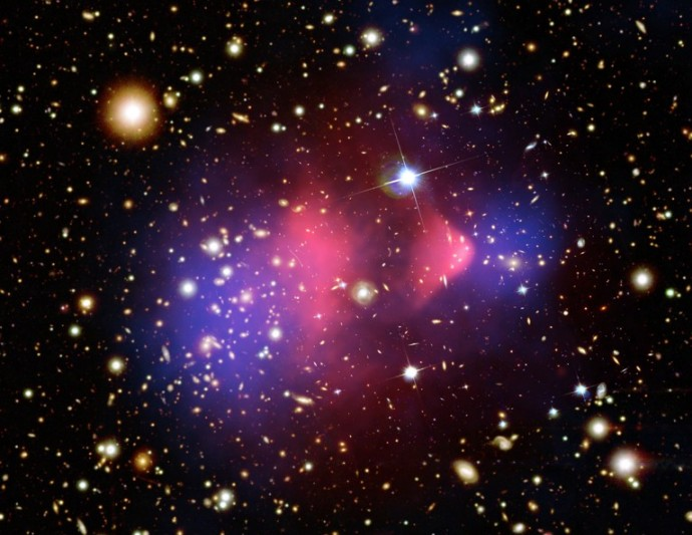
\includegraphics{figures/chapter_one/bullet_cluster.png}
	\caption{The Bullet Cluster of galaxies, from~\cite{bullet}}
	\label{fig:bullet_cluster}
\end{figure}

A good deal of information can be gleaned from a careful inspection of figure~\ref{fig:bullet_cluster}. The first thing to note is the separation of two populations of baryonic matter. In the visible wavelengths we observe the two subclusters with their galaxies largely undisturbed by their transit. The distance between galaxies in a cluster is larger than the characteristic size of a galaxy, thus a cluster is dominated by the star-less space between galaxies. When two galaxy clusters collide the chance of a direct collision between to galaxies is small, as the gaps for galaxies to slot between each other are larger than the galaxies themselves. Thus, we see that the two subclusters have been largely unaffected by their passage.

However, a respectable galaxy cluster contains far more than just galaxies. The majority of the mass comes from free hydrogen in the form of the hot x-ray gas. When two populations of gas pass through each other, they interact differently from galaxies. The gas interacts significantly as the two clouds pass through each other, which slows the gas down. Thus, as the two subclusters move away from each other post-collision, the x-ray gas will have lost some kinetic energy due to its interactions and will not leave the collision center as quickly as the stars and galaxies. This leads to a separation of the galaxies from the gas.

However, if a weak lensing study is performed on this cluster, it indicates that the lensing centers, and thus the greatest concentrations of mass, are centered around the galaxies, not the gas. This at first presents a dilemma, as the luminosities observed require that there be much more mass in gas than in galaxies. How, then, could the lensing be centered around somewhere the mass isn't? The answer is that there must be some hidden mass that accompanies each subcluster. Furthermore, we can note that this hidden mass didn't separate out with the gas, indicating that it doesn't experience significant self-interactions.

\section{Cosmological Evidence for Dark Matter}

While astrophysics tends to provide the prettier pictures, cosmology imposes more stringent numerical limits on dark matter and its distributions.

\subsection{Big Bang Nucleosynthesis (BBN)}

About a minute after the Big Bang, the universe had cooled sufficiently to allow nuclei to form and not be immediately broken apart due to the high ambient temperature. A good deal had happened in this minute, including the annihilation of all the antimatter with almost all the matter, creating the ocean of photons that is now the cosmic microwave background. It will prove convenient to define $\eta$ as the ratio between the number of baryons and the number of photons, or, as the number of photons is large, $\eta_{10} = 10^{10}\eta$. Neutrons and protons had just fallen out of numerical equilibrium due to their small difference in mass, and now existed in a ratio of about 1 neutron per 7 protons. Neutrons and protons first combined to make deuterium, then as the deuterium abundance increased, deuterium fused with deuterium to produce tritium and then with tritium to produce $^4$He. This epoch continued for just under half an hour, until expansion had driven particles far enough apart that collisions became infrequent and the temperature had decreased below the energy necessary to overcome the Coulomb repulsion between nuclei. Now, nearly all of the universe's neutrons were in helium due to its stability. Of the remaining few neutrons, most were in deuterium, with a few in $^7$Li. Due to its stability, the population of $^4$He depends very little on $\eta_{10}$, but deuterium is not strongly bound, so a smaller $\eta_{10}$ (more photons) means fewer deuterium nuclei. By measuring the primordial abundance of deuterium, this will admit a value of $\eta_{10}$ which will in turn indicate what percentage of the universe was baryons at this epoch.

\subsection{Cosmic Microwave Background (CMB)}

Pensias and Wilson were the first to turn a sensitive microwave telescope to the skies \cite{PenWil:1965a,PenWil:1965b}, and their discovery earned them the Nobel Prize in Physics in 1978. Now, the best measurements of the CMB come from satellites like WMAP and Planck. The basic data taken are nearly totally featureless and isotropic to a few parts per million as shown in Fig.~\ref{fig:cmb}a. If the average temperature of 2.7K is subtracted, a dipole term appears arising from the Sun's movement around the galaxy (Fig.~\ref{fig:cmb}b). In a sense, this indicates a favored reference frame for our universe, that is, one in which the observer is at rest relative to the CMB. If this dipole term is subtracted, the galactic contributions become clear (Fig.~\ref{fig:cmb}c). Subtracting this yields a density map of the universe when the CMB decoupled from the baryonic matter (about 380,000y after the Big Bang, Fig.~\ref{fig:cmb}d). Certain regions contain a slightly higher density than others, indicating a greater concentration of stuff. This temperature map can be expanded in the spherical harmonics and a power spectrum plotted. A cosmolical model is then fitted to this spectrum, and from this model various parameters of our universe can be extracted.

\subsection{Baryoacoustic Oscillations (BAO)}

\subsection{Structure Formation}

\section{Dark Matter in the universe today}

The burning question now is, what might dark matter be? The stuff must exist, so testable models should be proposed.

\subsection{Weakly Interacting Massive Particles (WIMPs)}

Observations (or lack thereof) of dark matter exclude interactions via electromagnetism and the strong force. However, this does not exclude weak interactions.

\subsubsection{Freezeout and the WIMP Miracle}

Supposing a population of particles existed in equilibrium with the rest of the universe at some early epoch (before BBN), as the univere expanded and cooled the production and annihilation reactions would begin to fall out of equilibrium. At some point, the universe was hot enough to allow for $\chi \bar{\chi} \leftrightarrow f \bar{f}$. However, once the temperature had dropped, the reverse reaction would become impossible, leaving $\chi \bar{\chi} \rightarrow f \bar{f}$. Eventually even this would become impossible, leaving no allowed reactions.

\subsection{Massive Compact Halo Objects (MACHOs)}

The limits on non-baryonic matter deriving from the CMB rely on the lack of detectable interaction with the CMB. However, there are more things that interact with the CMB in ways that our telescopes aren't sensitive enough to detect. The MACHO theory posits a dark matter halo filled with massive compact baryonic objects such as unowned Jupiter-sized planets, dwarfs, and small, quiet black holes. Such objects would radiate only very weakly, which would be very difficult for telescopes to directly identify. Detection of these objects is principally done through observation of micro-lensing events, where a MACHO passes in front of a background star in such a way that the gravitational lensing acts to greatly magnify the star. Modelling is then done to identify both the location and mass of the lensing object. These events have been observed but the frequency with which they happen only admits []\% of the required mass of dark matter~\cite{}.

\subsection{Axions}

Originally proposed as a solution to the strong-CP problem, axions were suggested to be dark matter candidates in [].

\subsection{Neutrinos}

The elephant in the room at this point is neutrinos. Neutrinos only interact via the weak and gravitational forces, and should be dead ringers for dark matter. Why, then, are we still looking? The answer lies in temperature. Due to the extremely low mass of neutrinos, any amount of energy greater than a few eV is sufficient to make the neutrino ultrarelativistic. Additionally, there are no mechanisms whereby a lot of neutrinos can lose a lot of energy. So, once a neutrino is created, it will tend to hold on to whatever energy it has.

Now, if the early universe was filled with ultrarelativistic matter, the structure formation we observe today could not have occurred. Any overdensity of ultrarelativistic matter will have a greater outflux than influx, which will tend to smoothe out any tendency of matter to clump under the influence of gravity. During the period of primary structure formation, most of the universe's neutrinos would have been ultrarelativistic, and so if they had been a significant component of dark matter the universe today would have a much more uniform distribution of mass, as opposed to the observed scattered delta functions. Additionally, Planck limits $\Omega_\nu$ to $<$ value~\cite{}, which is far too low to be a dominant component.

%\end{document}